\chapter{Privacy Analysis}
\label{ch:PrivacyAnalysis}

The Privacy Analysis represents the analysis stage in the MAPE-K feedback loop (\autoref{sec:Foundations:mape}). The goal is to check whether the runtime model contains any deployment related privacy violations. The privacy concept, described in \autoref{ch:PrivacyConcept}, states that privacy analysis consist of two major tasks. First, the correct privacy categorization for each software components needs to be determined. Second, the deployment evaluation, based on the deployment rules, defined in \autoref{sec:PrivacyConcept:deploymentrules}, needs to be performed.

The remaining chapter is divided into a theoretical part (\autoref{sec:PrivacyAnalysis:theory}), a component categorization part (\autoref{sec:PrivacyAnalysis:categorization}), a deployment evaluation part (\autoref{sec:PrivacyAnalysis:deployment}) and the implementation part (\autoref{sec:PrivacyAnalysis:implementation}).


\section{Analysis Theory}
\label{sec:PrivacyAnalysis:theory}

The exclusive source of information for the privacy analysis is the systems PCM Privacy runtime model. For an efficient analysis one first need to identify the minimal required information and substitute them, depending on the available sources.


\subsection{Required information}
In the context of Privacy Analysis there is a minimum of two pieces of information which are required for privacy analysis:

\begin{table}[h]
	\centering
	\begin{tabular}{r | l}
		\hline
		\textbf{\#} & \textbf{Required information for privacy analysis}\\
		\hline
		M1 & Information on components privacy level \\
		M2 & Information on components geo-location \\
		\hline
	\end{tabular}
	\caption{Minimal information for privacy analysis}
	\label{tab:pa_minimal_info}
\end{table}

Usually \textit{M1} and \textit{M2} is not directly available. As a consequence other ones must substitute these, while containing the same information. A suitable substitution, differs based on the sources and their contained information.

The used PCM Privacy meta-model provides a categorization of the communicated information between component interfaces. This enables a component classification, based on the most critical communication with another component. As a result, a components privacy level can be determined without knowing its exact purpose, analysing any inner processes or knowing the exact data-flow. So, $M1$ gets substituted by information about inter interface communication and its privacy categorization.

In order to get an information equivalent of $M2$, a components host must be determined, as well as that hosts geo-location. The PCM Privacy model provides these information. However, it is spread over multiple models. As a result we require only four pieces of information (\autoref{tab:iobserve_information}), compared to R-PRISs six pieces of information (\autoref{tab:rpris_information}).

\begin{table}[h]
	\centering
	\begin{tabular}{r | l}
		\hline
		\textbf{\#} & \textbf{Required information to carry out runtime check}\\
		\hline
		I1 & Interactions of two components per interface \\
		I2 & Information on component deployments on physical resources \\
		I3 & Geo-location information of physical resources \\
		I4 & Data Privacy categorization per interface communication \\
		\hline
	\end{tabular}
	\caption{iObserves information for runtime privacy checks}
	\label{tab:iobserve_information}
\end{table}

\subsection{Data-flow direction}
\label{sec:PrivacyAnalysis:theory:dataflow}
Usually component interfaces are categorized into providing and requiring interfaces. Interface connections are made between a pair of required and provided interfaces of the same type. This suggests a certain data- and control-flow direction. This is a wrong assumption. While there are cases, when the control-flow can be derived from this structure, the data-flow is completely independent from this categorization.

For example a database component (usually) only has provided interfaces. These interfaces allows the user to store and retrieve data from the database and therefore contains getter and setter methods. This means, there is no data-flow direction for the whole interfaces, since the data needs to "flow" into both directions. Note, that we are explicitly speaking of an interface as a whole, since individual methods can have a data-flow direction.

Information passed through an interface are available on the providing and requiring component. In other terms, if an component connector got categorized as \textit{Personal}, information of this type are available in both components. These components need to get categorized accordingly.

\subsection{Joining data streams}
\label{sec:PrivacyAnalysis:theory:jds}
In \autoref{sec:PrivacyConcept:deploymentrules} we elaborated on the danger of two \textit{Personally Identifiable Information} (Type 1) data streams, from two sources, joining on a single server. In such a case, the combination of these data streams could lead to personal, privacy relevant data. (Compare \autoref{enum:deployment_rules}, Rule 4). This concept applies on the described deployment level and also on the component categorization process.

While on deployment level, the information streams are not actively merged, this is a realistic possibility on the component categorization level. So the argument of applying an overestimation is not valid and this scenario must be taken seriously. In the following this special case will be refereed to as \textit{joining data streams} (short: JDS). In the following section, a couple of categorization and deployment examples will help clarifying this scenario.


\section{Component categorization}
\label{sec:PrivacyAnalysis:categorization}

The component categorization requires two tasks. The initial categorizing of every component and the "upcasting" of components with join data streams.

The initial data privacy level of a component is equal the components most critical communication level (see \autoref{sec:PrivacyAnalysis:theory:dataflow}). Example \autoref{fig:example_categorization:init} shows the components data privacy level after the initial categorization phase.

\begin{figure}[h]
	\centering
	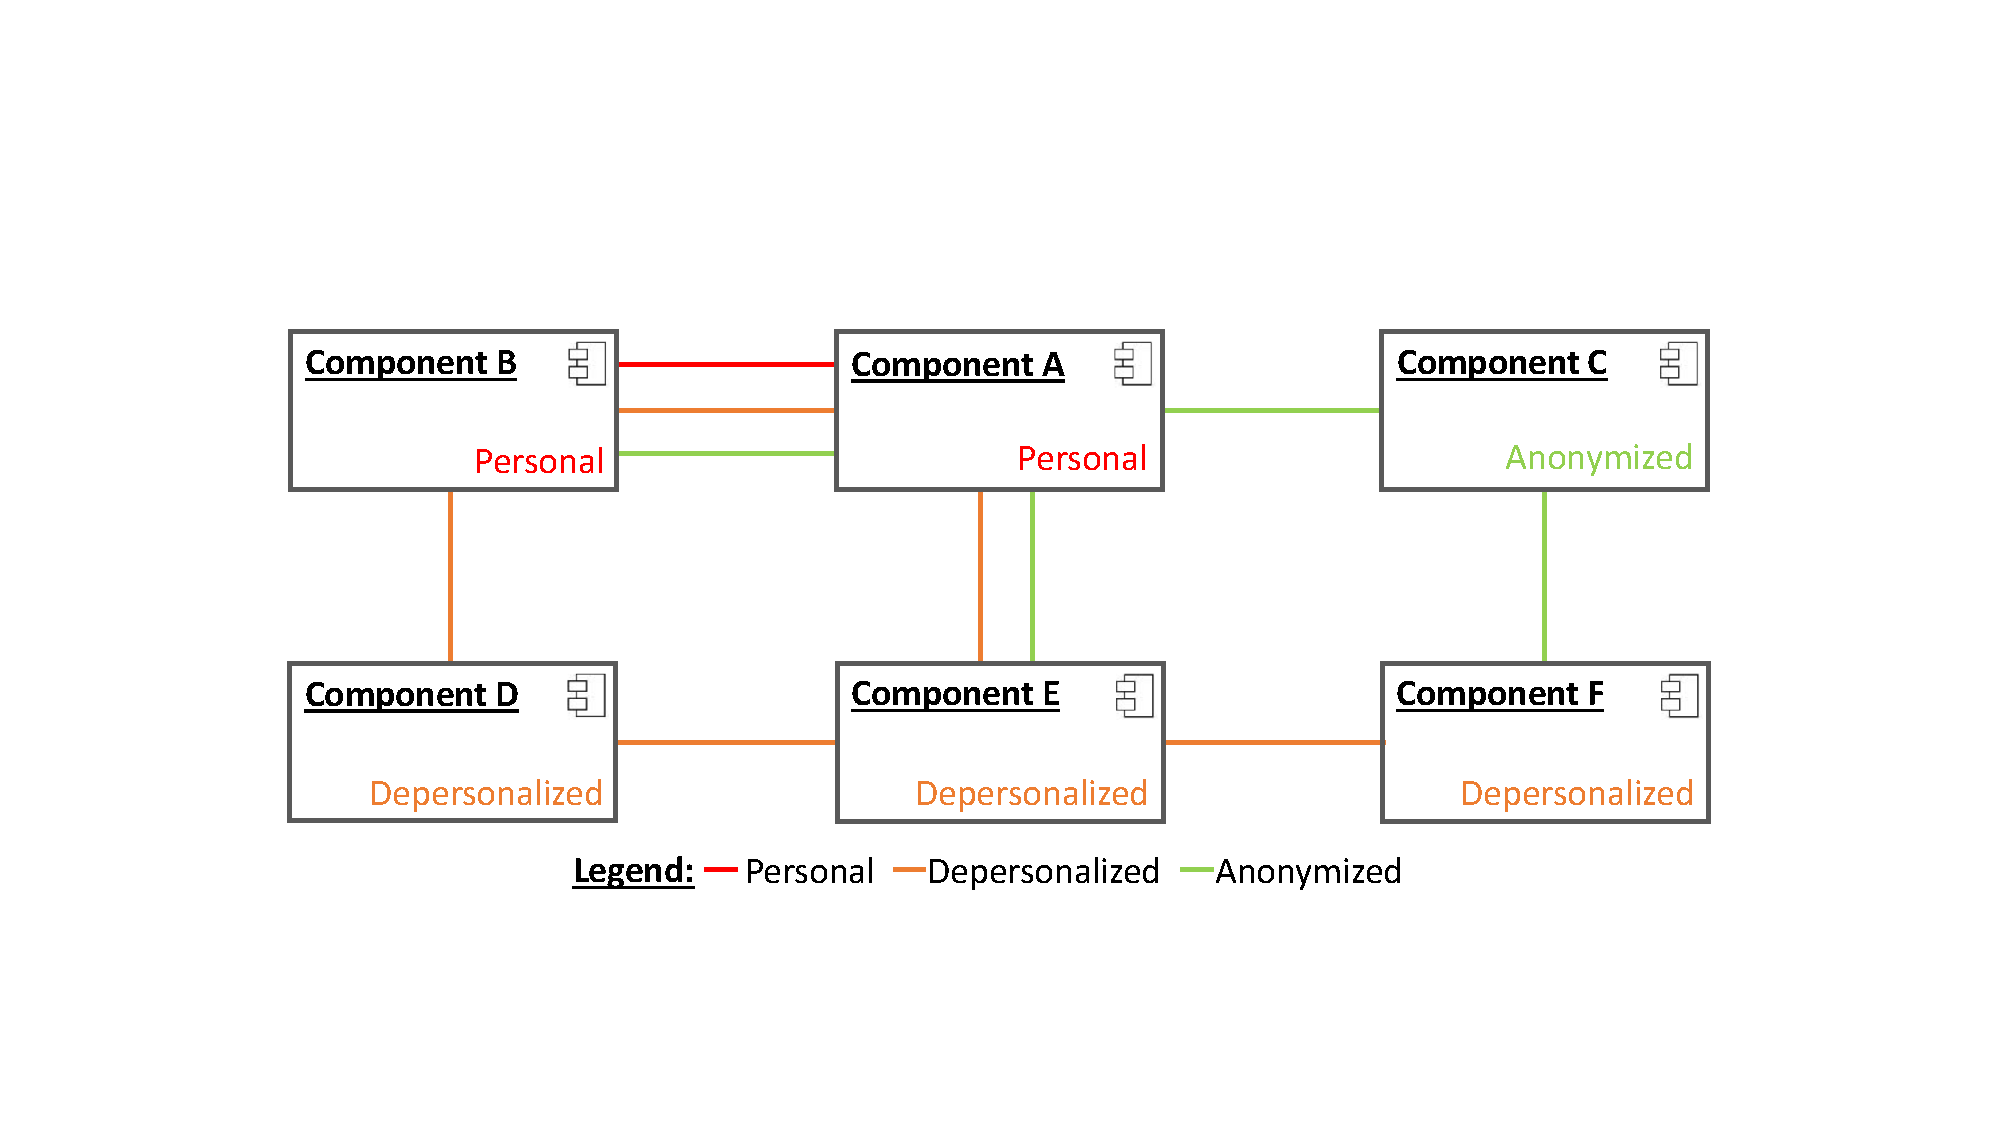
\includegraphics[trim = 35mm 40mm 40mm 45mm, clip, width=0.75\textwidth]{graphs/component_categorization_examples_initial}
	\caption{Initial component categorization}
	\label{fig:example_categorization:init}
\end{figure}

The second phase analyses the system for joining data streams. \autoref{fig:example_categorization:base} continues the initial example), and shows the result of the second phase. In comparison to the initial categorization, component D and E get "upcasted" and gain a \textit{Personal} - more critical - data privacy categorization. This is due to the fact, that component D and E have a connection onto two personal data sources (Component A and B).

\begin{figure}[h]
	\centering
	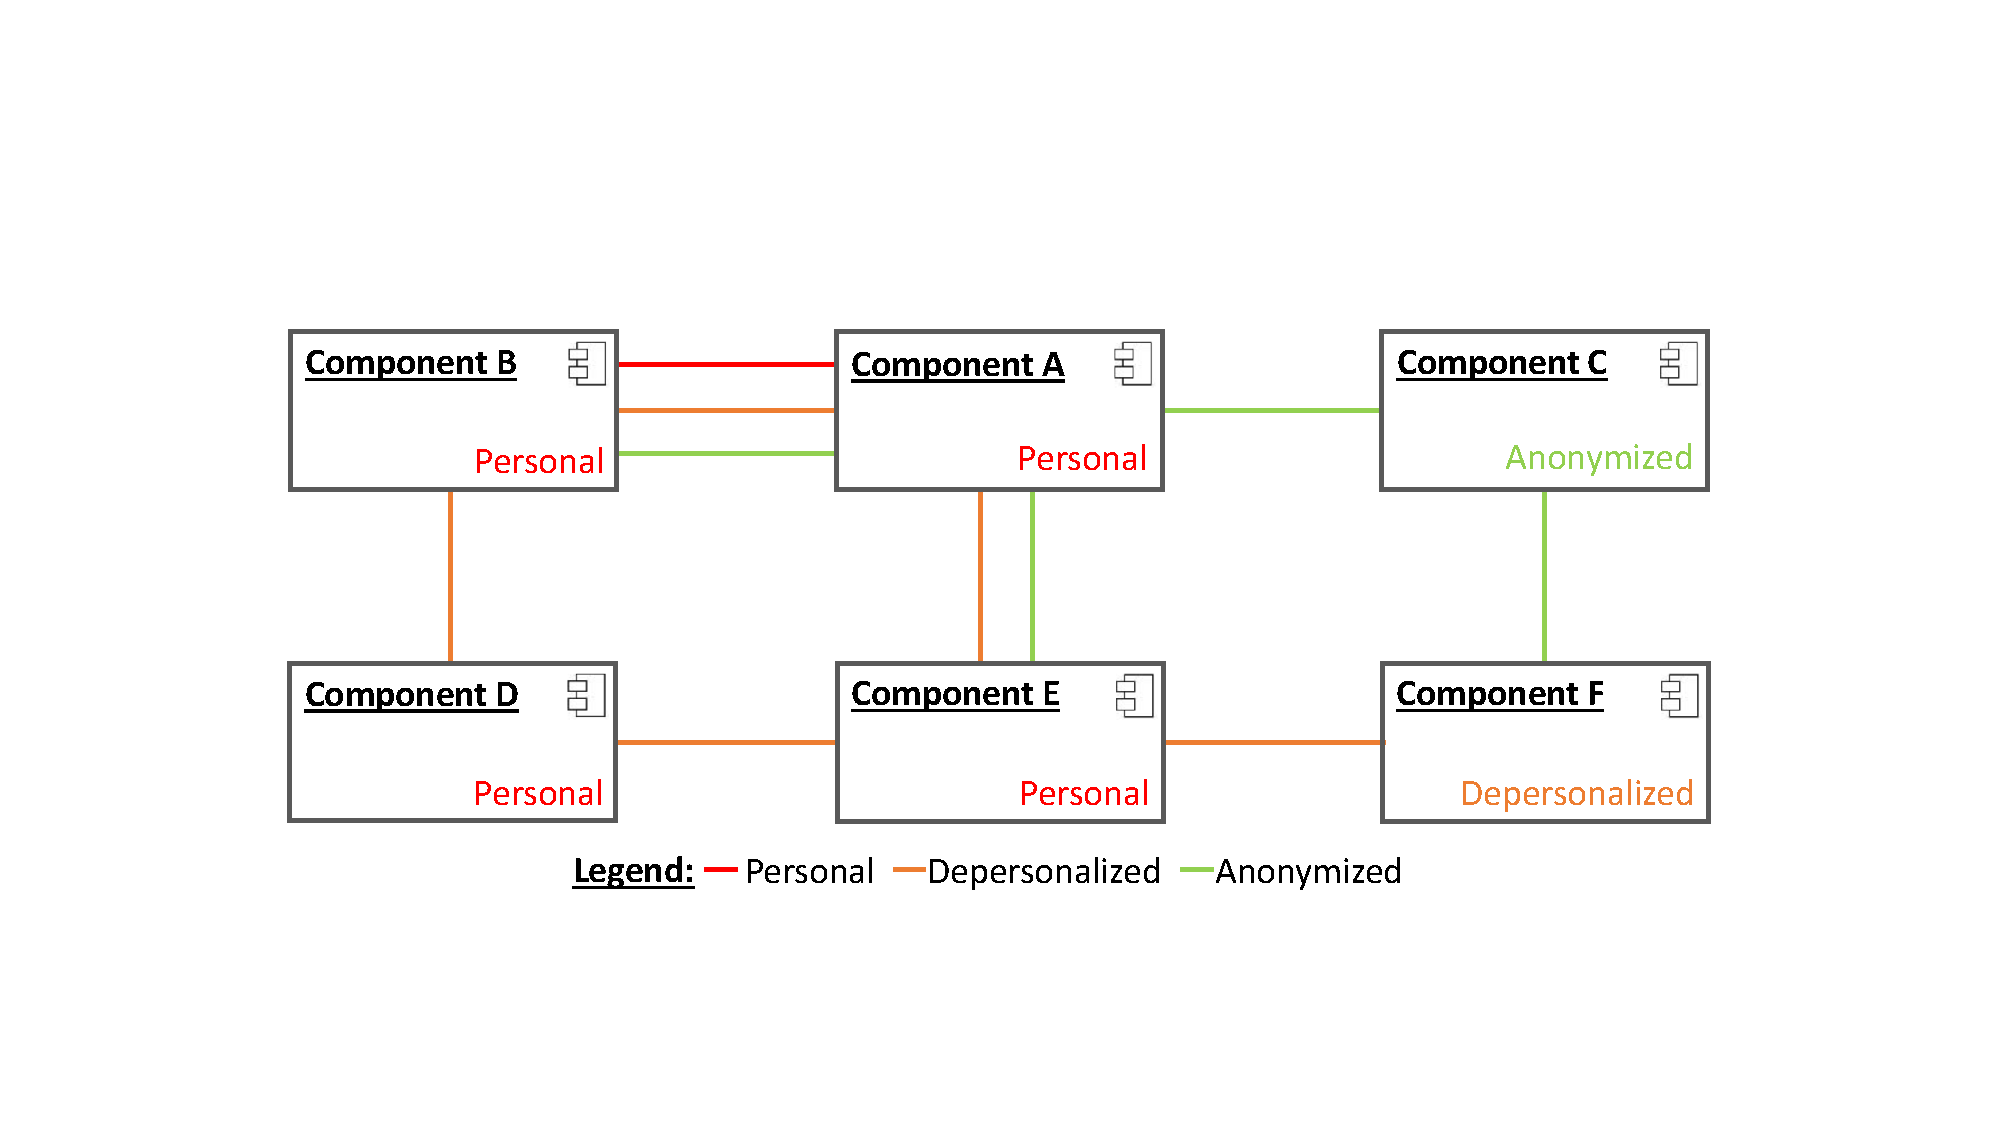
\includegraphics[trim = 35mm 40mm 40mm 45mm, clip, width=0.75\textwidth]{graphs/component_categorization_examples_upcast_base}
	\caption{Post categorization analysis - basic example}
	\label{fig:example_categorization:base}
\end{figure}

Two special cases are shown in \autoref{fig:example_categorization:advanced}. So does component D gets a personal data marking even though it has only one other component as data source. However, it has two individual connections to component B, which could contain a joining data stream, since B has a personal categorization.

\begin{figure}[h]
	\centering
	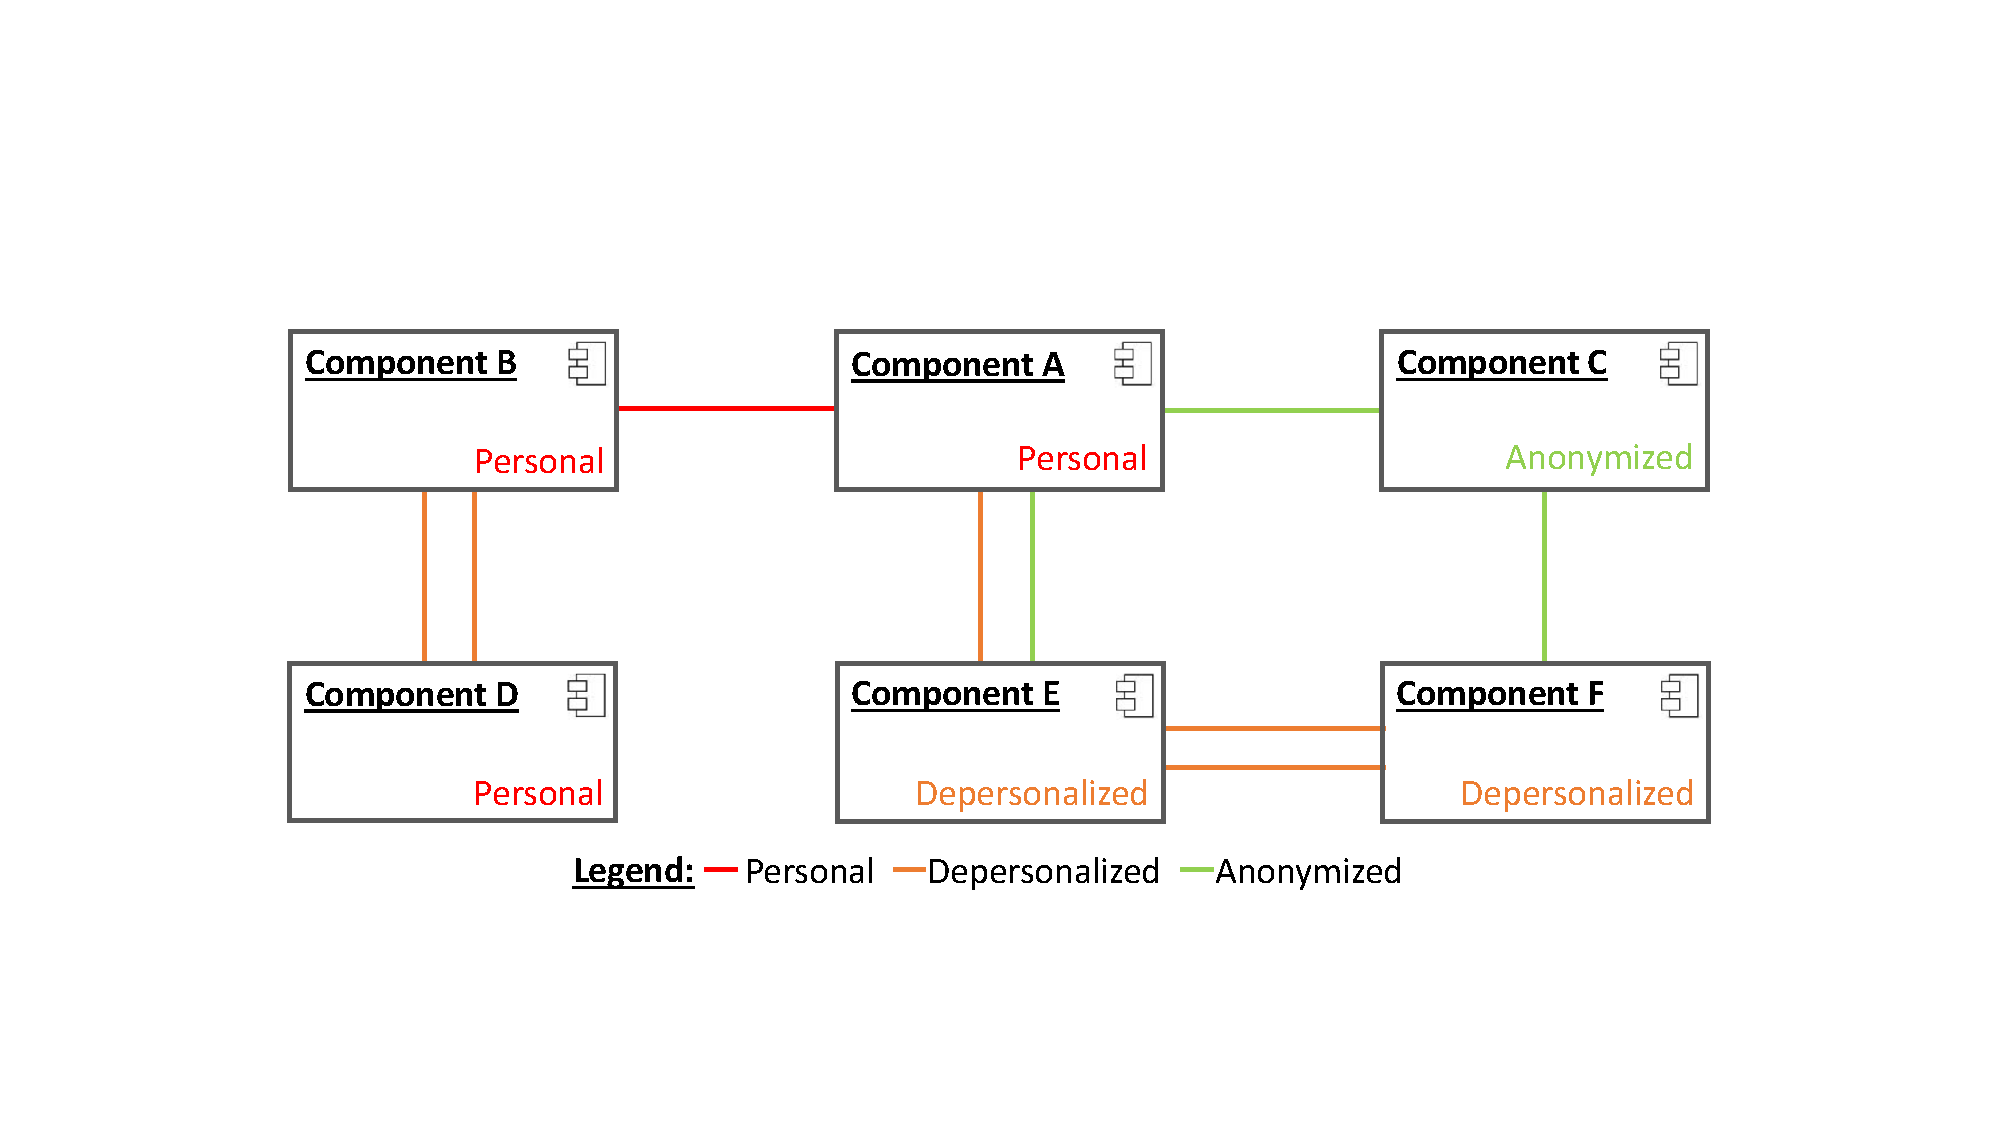
\includegraphics[trim = 35mm 40mm 40mm 45mm, clip, width=0.75\textwidth]{graphs/component_categorization_examples_upcast_advanced}
	\caption{Post categorization analysis - advanced example}
	\label{fig:example_categorization:advanced}
\end{figure}

Component F doesn't get an "upcast" since it can only contain privacy relevant data that are already present on component E. And component E has a depersonalized categorization. All anonymized categorized connections and components are ignored, since they don't contain any privacy related information.


\section{Deployment analysis}
\label{sec:PrivacyAnalysis:deployment}

The deployment analysis' goal is to find out whether the current deployment is privacy compliant. The rules for a privacy compliant deployment were described in \autoref{sec:PrivacyConcept:deploymentrules}.

\autoref{fig:example_deplyoment_eval} shows an illegal deployment. The deployment of Component A and B is obviously valid, due to its deployment on a "save" geo-location. Component C and F are also legally deployed, since both components share a single communication edge onto privacy relevant information and the "joining data streams" situation does not apply. Server\#2, however, hosts an illegal deployment. Component D and E have different single data sources edges and can therefore save, process or transmit data, which can combine to privacy relevant data.

\begin{figure}[h]
	\centering
	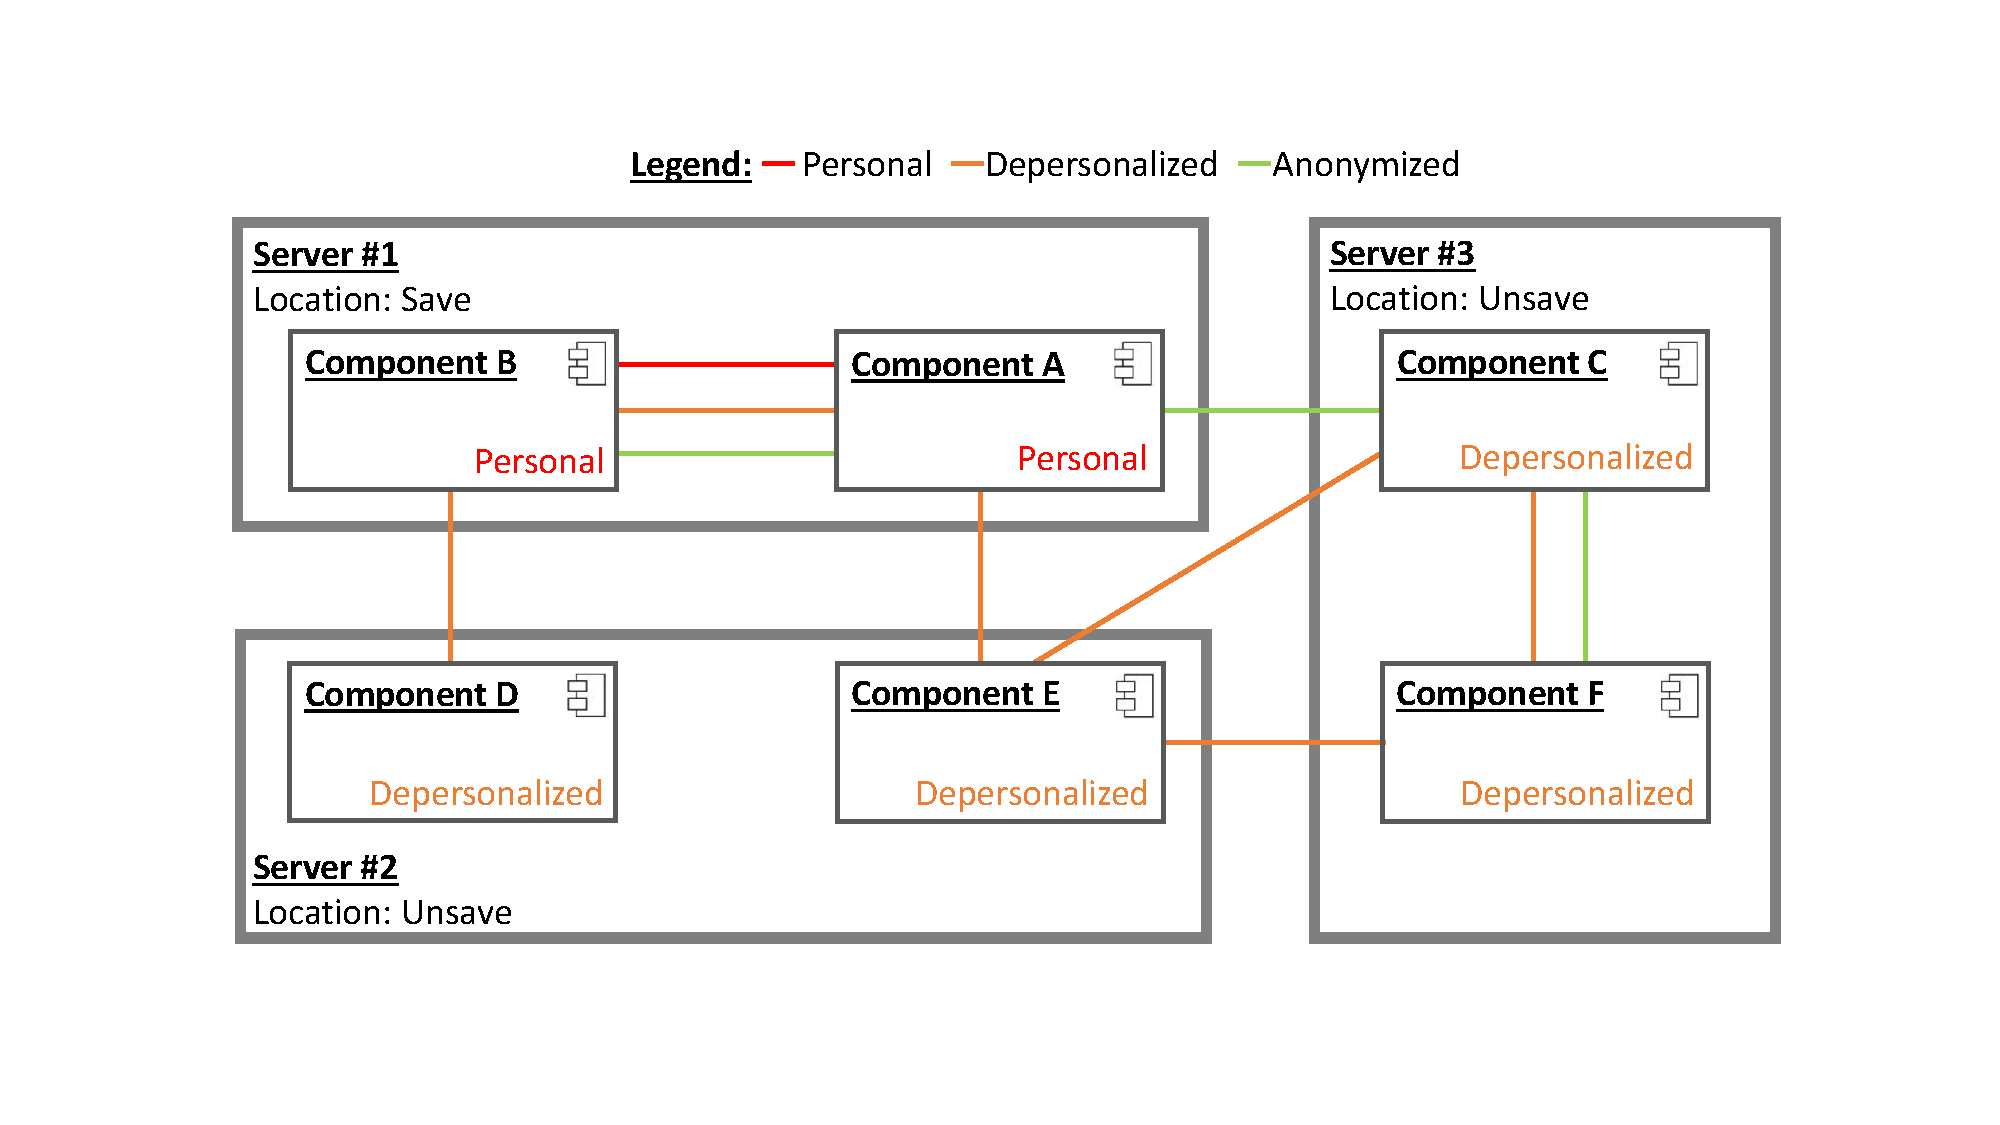
\includegraphics[trim = 35mm 30mm 30mm 25mm, clip, width=0.85\textwidth]{graphs/deployment_example_implementation_eval}
	\caption{Deployment analysis example}
	\label{fig:example_deplyoment_eval}
\end{figure}


\section{Privacy Analysis implementation}
\label{sec:PrivacyAnalysis:implementation}

The PCM meta-model defines multiple models, each providing knowledge about a certain aspect of the target system (see \autoref{fig:pcm_info_spread}). This is not suited for an efficient privacy analysis and therefore requires an information preprocessing. So the implementation is spread over three steps:

\begin{enumerate}
	\label{enum:algorithm_steps}
	\setlength\itemsep{0em}
	\item build efficient data structure
	\item categorize components
	\item analyse deployment
\end{enumerate}


\subsection{Information preprocessing}

In the first algorithm phase, all informations $I1$ to $I4$ are extracted from the different models. $I1$ and $I4$ is part of the System models Assembly Connector Privacy. Where $I1$ consist of the Providing Assembly Context and the Requiring Assembly Context. $I4$ is the Data Privacy Level. $I3$ is a field in the Resource Container, which represents a server in the Resource Environment model. The Allocation model contains $I2$ in Allocation Contexts, which provide a mapping of an Assembly Contexts on a Resource Containers.

After extracting all required information, the basic data privacy level for every component/Assembly Context is calculated by applying the most critical privacy level from the corresponding Assembly Connectors.

As last step of the preprocessing, the data are reassembled by constructing a sufficient graph (\autoref{fig:privacy_graph_mm}). The graph is a simple, more direct representation of host-component-allocation structure from the PCM model. The graph contains two types of nodes: the DeploymentNode, a host representation, and the ComponentNode, a component representation. The data streams/interfaces are represented by the ComponentEdge:

\begin{figure}[h]
	\centering
	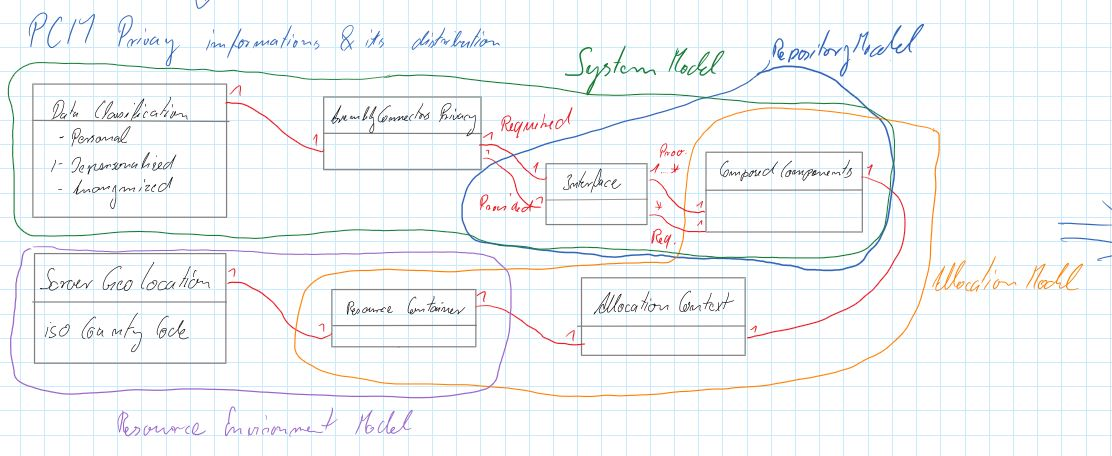
\includegraphics[width=0.5\textwidth]{pictures/pcm_info_spread}
	\caption{PCM Privacy information spread}
	\label{fig:pcm_info_spread}
\end{figure}

\begin{figure}[h]
	\centering
	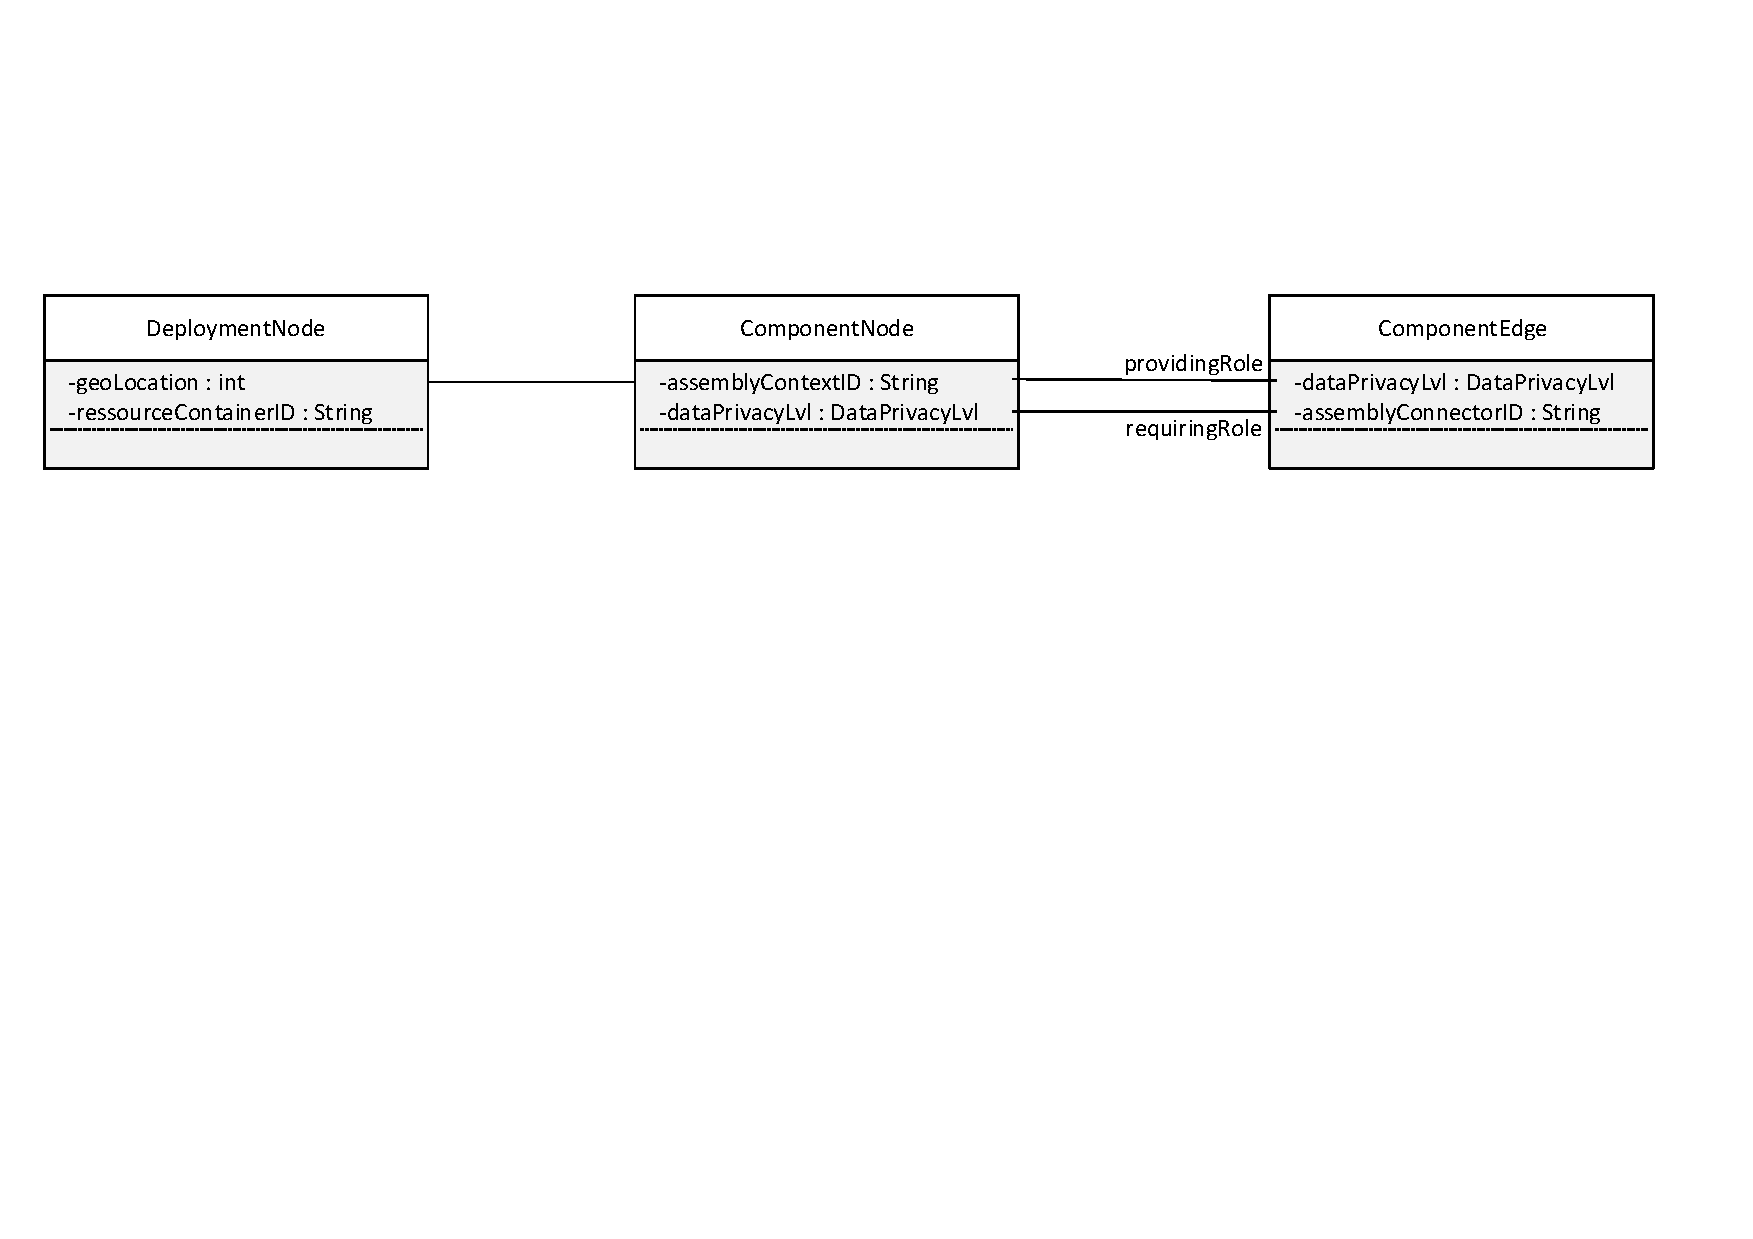
\includegraphics[trim = 00mm 120mm 15mm 50mm, clip, width=0.85\textwidth]{pictures/modelGraph_metamodel}
	\caption{Graphs meta-model for Privacy Analysis}
	\label{fig:privacy_graph_mm}
\end{figure}


\subsection{Component categorization implementation}

The second phase of the privacy analysis algorithm finalizes the component categorization. As described in \autoref{sec:PrivacyAnalysis:categorization}, joining data streams need to be found and fitting components' data privacy level corrected.

The algorithm (Algorithm \ref{algo:comp_categ}) searches for depersonalised-marked connections from one personal categorized component to another. It uses a \textit{deep search first} approach, while never using an edge twice. Note, that once a joining data stream is found, the involved components are appended to the list of personal components.

\begin{algorithm}[h]
	\caption{Component categorization algorithm}
	\label{algo:comp_categ}
\begin{algorithmic}[1]
	
	\State List of Components $components$
	\State Set of Edges $usedEdges$ 
	\State
	\Procedure{StartCategorization}{List<Components> $components$}\State
		$personalComponents\gets components with PrivacyLvl == PERSONAL$
		\ForAll{$personalComponent\gets Components$}\State
			\Call{clear}{ $usedEdges$ }\State
			\Call{TraverseComponent}{ $personalComponent$ }
		\EndFor
	\EndProcedure \State
	
	\Function{TraverseComponent}{Component $component$}\State
		$dePersonalEdges\gets component.$\Call{GetEdges}{} with $PrivacyLvl == DEPERSONAL$
		\ForAll{$edge\gets dePersonalEdges$}\State
			\If{$usedEdges.$\Call{Contains}{ $edge$ }} \State 
				\Call{Continue}{}
			\Else \State
				$usedEdges.$\Call{Add}{ $edge$ } \State
				$edgeParnter\gets edge.$\Call{GetEdgePartner}{ $component$ } \State
				
				\If {$edgeParnter.PrivacyLvl == PERSONAL$} \State
					\Return $edgeParnter$
				\Else \State
					$secondSource\gets$ \Call{TraverseComponent}{ $edgeParnter$ }
					\If{$secondSource \neq PERSONAL$} \State
						$component.PrivacyLvl\gets PERSONAL$ \State
						$components.$\Call{Add}{ $component$ } \State
						\Return $secondSource$
					\EndIf
				\EndIf 
			\EndIf
		\EndFor \State
		\Return Null
	\EndFunction
\end{algorithmic}
\end{algorithm}



\subsection{Deployment analysis implementation}

The final privacy analysis phase is the deployment evaluation. The base analysis is very simple, since it simply checks whether every as personal categorized component is deployed on an as save considered geo-location. The a geo-location is considered as save, when it is contained in the save-geo-location list. When a server is located in an un-save geo-location and contains more then one depersonalised component, an extensive analysis for joining data streams has to be made. This extensive analysis is described in Algorithm \autoref{algo:deployment_analysis}.

The Algorithm works similar to Algorithm \ref{algo:comp_categ}. Initially, it extracts all as depersonalised categorized components on the server. These components have to form a transitive hull and share a single depersonalised communication link to a single personal component. The algorithm uses a \textit{deep search first} approach to traverse through the components. If a second link to a personal component is found or not every depersonalised component on the server is reached, the deployment is illegal.

Note, that anonymized categorized components and edges can be ignored during analysis. Also, a server won't contain any personal marked component since such a deployment would be automatically illegal due to the servers un-save geo-location.


\begin{algorithm}[h]
	\caption{Deployment analysis algorithm}
	\label{algo:deployment_analysis}
	\begin{algorithmic}[1]
		
		\State Set of Components $compToReach$
		\State Set of Edges $usedEdges$
		\State Edge $dataSourceEdge$
		\State
		\Procedure{ExtensiveAnalysis}{Server $server$}
			\State $compToReach\gets server.$\Call{GetComponents}{} with $PrivacyLvl == DEPERSONAL$
			\State $dataSourceEdge \gets Null$
			\State $startComp\gets compToReach.$\Call{GetAny}{}
			\State {clear}{ $usedEdges$ }
			\State $singlePersonalDataSource\gets $\Call{TraverseComponent}{startComp}
			\State \Return $singlePersonalDataSource$ AND $compToReach.$\Call{IsEmpty}{} 
		\EndProcedure \State
		
		
		\Function{TraverseComponent}{Component $component$}
		\State $compToReach.$\Call{Remove}{ $component$ } 
		\State $dePersonalEdges\gets component.$\Call{GetEdges}{} with $PrivacyLvl == DEPERSONAL$\State
		
		\ForAll{$edge\gets dePersonalEdges$}
			\If{$usedEdges.$\Call{Contains}{ $edge$ }}
				\State \Call{Continue}{}
			\Else 
				\State $usedEdges.$\Call{Add}{ $edge$ } 
				\State $edgeParnter\gets edge.$\Call{GetEdgePartner}{ $component$ } 
				\State
				\If {$edgeParnter.PrivacyLvl == PERSONAL$}
					\If {$dataSourceEdge == Null$} 
					 	\State $dataSourceEdge \gets edge$
				 	\Else 
					 	\State \Return False
				 	\EndIf
				\Else \State
					$singleDataSource\gets$ \Call{TraverseComponent}{ $edgeParnter$ }
					\If{$singleDataSource$} 
						\State \Return False
					\EndIf
				\EndIf 
			\EndIf
		\EndFor 
		\State \Return True
		\EndFunction
	\end{algorithmic}
\end{algorithm}


